\section{A basic machine learning problem: image classification}
%The ultimate goal of supervised learning algorithms is to classify the data into correct categories.
%Classification is a very basic  yet important problem
%which is based on a training set of data containing observations (or instances) whose category memberships are known. An example is to classify a given email into ``spam" or ``non-spam" classes. Assigning a diagnosis to a given patient based on the observed characteristics of the patient (such as gender, blood pressure, presence or absence of certain symptoms, etc.) would be another example. To understand what it the image classification problem, let us propose the following question:
Classification problem is a very important part of machine learning. Its goal is to determine which class a new data belongs to based on a set of training data whose class is known. For example, in mail management, classifying an e-mail as ``spam" or ``non-spam" is a typical binary classification problem, and the classification of credit rating of credit card customers by banks belong to multiple classification problems. More specifically, in order to understand image classification problem, let us pose the following question:


\begin{itemize}
	\item Given a set of images of cat, dog and rabbit, how does a machine classify the three different classes?
\end{itemize}

\begin{figure}[H]
	\begin{center}
		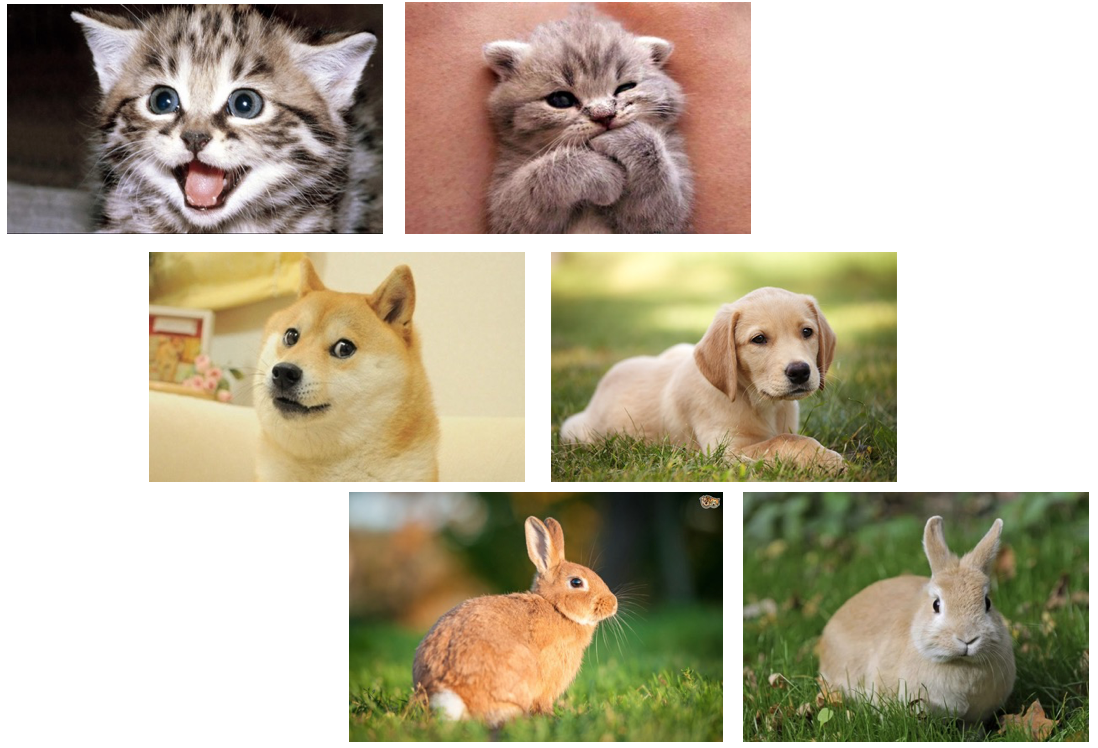
\includegraphics[width=.4\textwidth, height=.2\textheight]{figures/cat-dog-1.png}
	\end{center}
	%	\caption{}
\end{figure}

\break

First of all, we introduce how an image is represented on computer. Mathematically, {gray-scale image can be considered as a matrix  in $ \mathbb{R}^{n_0\times n_0}$ shown below, where the left one is the image from human vision and the right one is the matrix represented in computer. Each entry in this $ \mathbb{R}^{n_0\times n_0}$ corresponds to the value of a pixel belong to $[0,255]$.
	\begin{center}
		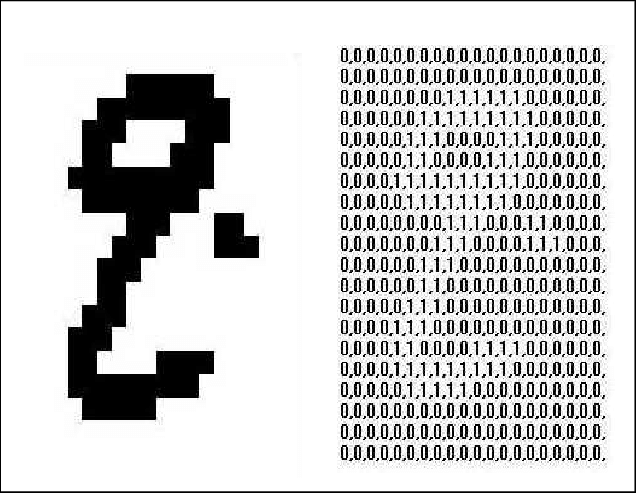
\includegraphics[width=.4\textwidth, height=.2\textheight]{6DL/figures/gray-1.png}
	\end{center}
	%The next figure shows different results from: {human vision and computer representation}:{\color{red}Lian comments: should it be a 3D tensor?}
	%\begin{figure}[H]
	%	\begin{center}
	%		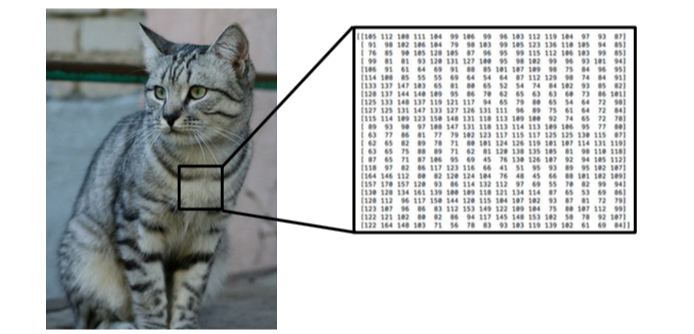
\includegraphics[width=.4\textwidth, height=.2\textheight]{figures/ImagePixels.png}
	%	\end{center}
	%\end{figure}
	A color image can be taken as 3D tensor (matrix with $3$ channels (RGB)) in $ \mathbb{R}^{n_0\times n_0 \times 3}$
	\begin{center}
		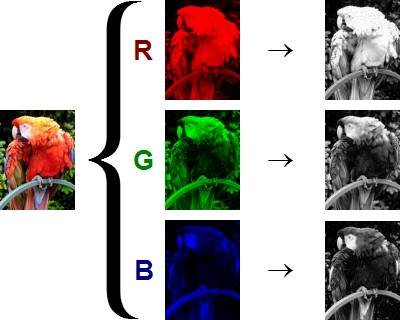
\includegraphics[width=.4\textwidth, height=.2\textheight]{6DL/figures/corlor-1.png}
	\end{center}
	
	%\begin{itemize}
	%	\item An image is just a big grid of numbers between [0, 255]
	%	\begin{itemize}
	%		\item e.g. 800$\times$600$\times$3 (3 channels RGB)
	%	\end{itemize}
	%\end{itemize}
	
	
	\break
	
	Then, let us think about the image classification problem of cat, dog and rabbit. Each image is a big vector of pixel values, for example
	$$ d=1280\times720\times 3  (\text{width} \times \text{height} \times \text{RGB channel}) \approx 3\text{M},$$
	which can be considered as a point $x \in \mathbb{R}^d$. The question becomes: given 3 different sets of points (cat, dog and rabbit) in $\mathbb{R}^d$, how does a machine classify them?
	\begin{figure}[H]
		\begin{center}
			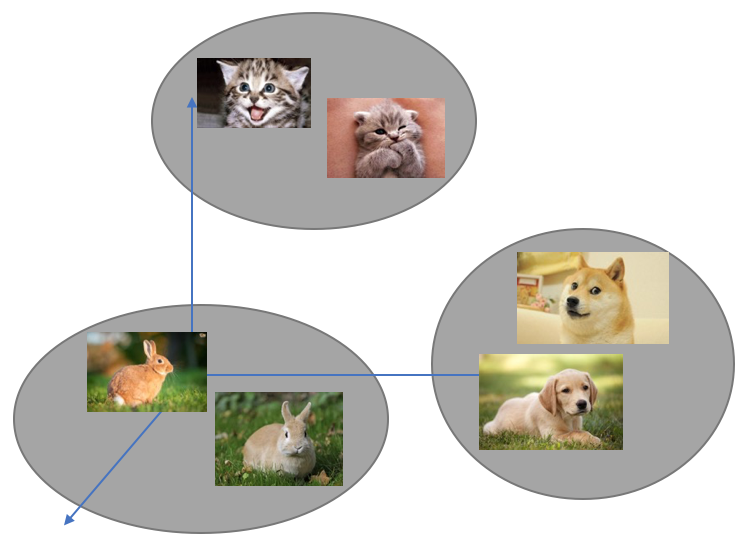
\includegraphics[width=.3\textwidth, height=.3\textwidth]{figures/cat-dog-2.png}   \quad \quad  \quad \quad
			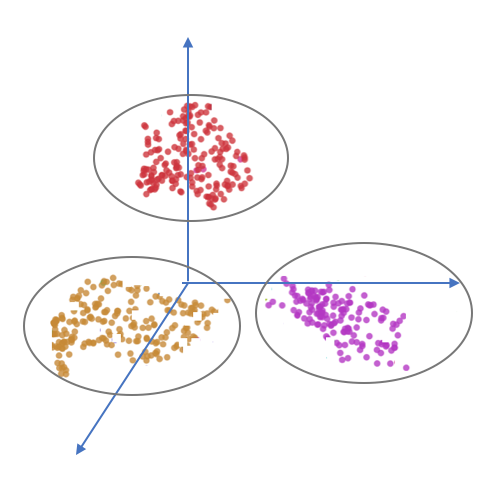
\includegraphics[width=.3\textwidth, height=.3\textwidth]{figures/cat-dog-3.png}
		\end{center}
	\end{figure}
	
	\noindent To answer this question, we consider a mathematical problem: Find $f(\cdot; \bm \theta): \mathbb{R}^d \to \mathbb{R}^3$ such that:
	$$
	f(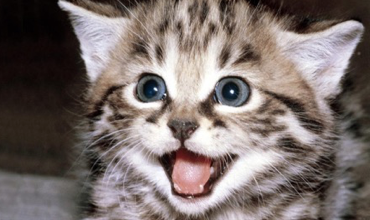
\includegraphics[width=.07\textwidth]{figures/cat.png}; \Theta)
	\approx \begin{pmatrix}
	1\\ 0 \\ 0
	\end{pmatrix}
	,\quad
	f(
\includegraphics[width=.07\textwidth]{figures/dog.png}; \Theta)
	\approx \begin{pmatrix}
	0\\ 1 \\ 0
	\end{pmatrix}
	,\quad
	f(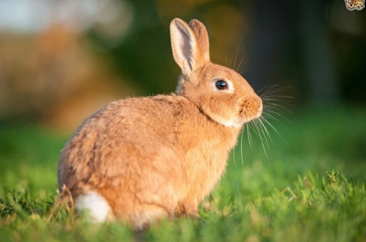
\includegraphics[width=.07\textwidth]{figures/rabbit.png};
	\Theta) \approx
	\begin{pmatrix}
	0\\ 0 \\ 1
	\end{pmatrix}
	.
	$$
	$f(\cdot; \bm \theta)$ maps a given image to a 3-dimensional vector, which is a probability distribution  $\begin{pmatrix}
	p_1\\ p_2 \\ p_3
	\end{pmatrix}$
	, where $p_1, p_2, p_3$ are probabilities of the given image being cat, dog, rabbit, respectively. For example
	
	$$
	f(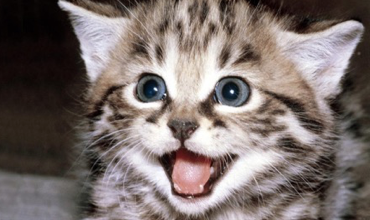
\includegraphics[width=.07\textwidth]{figures/cat.png}; \bm \theta)
	=
	\begin{pmatrix}
	0.7\\ 0.2 \\ 0.1
	\end{pmatrix}
	\quad \Longrightarrow \quad 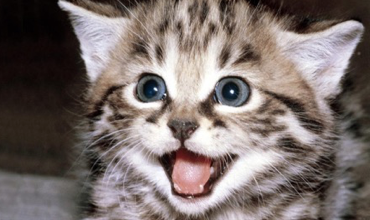
\includegraphics[width=.07\textwidth]{figures/cat.png}= {\rm cat}.
	$$
	$f$ is a classifier that can be used to classify what a given image is.
	
%%	As an example, we introduce the image classification of cat, dog, rabbit above. More general, classification problem is to find some curves or surfaces to separate some sets of data. As examples, the following two images show how a circle and a curve separate different sets of points
%%	\begin{figure}[H]
%%		\begin{center}
%%			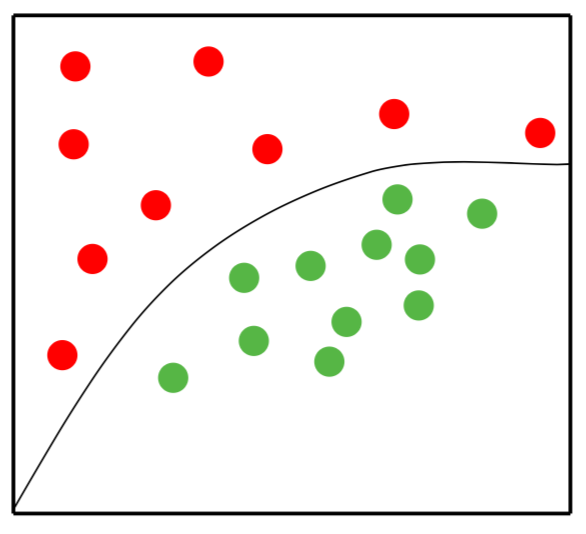
\includegraphics[width=1.5in]{NLinearS1.png}  \quad
%%			\quad  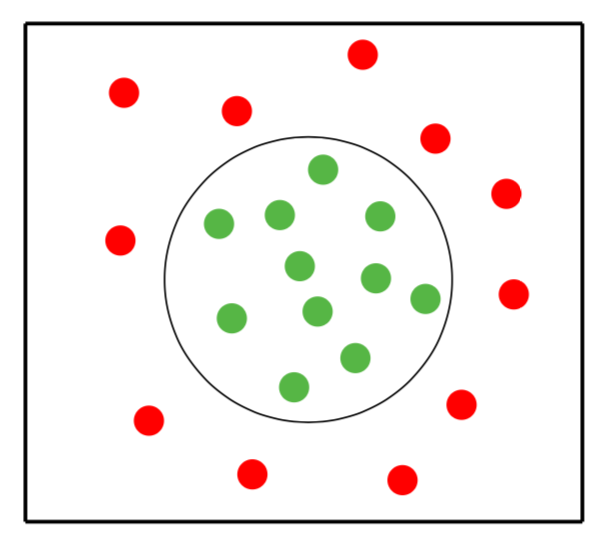
\includegraphics[width=1.5in]{NLinearS2.png}
%%		\end{center}
%%	\end{figure}
%%	\noindent It begins with a data set (training data)
%%	$$
%%	D := \{(x_j, y_j)\}_{j=1}^N,
%%	$$
%%	and
%%	$$
%%	A = \{ x_1, x_2, \cdots, x_N\} \quad \text{with} \quad A = A_1\cup A_2\cup \cdots \cup A_k, ~A_i\cap A_j = \emptyset, \forall i \neq j,
%%	$$
%%	where $A_1,...,A_k$ are a collection of subsets of A,
%%	$y_j \in \mathbb{R}^{k}$ is the label of data $x_j$ with
%%	$y_j[i]$ as the probability of $x_j$ in class $i$ or $x_j \in A_i$. If $x_j \in A_{i_j}$, we often choose
%%	\begin{equation}\label{key}
%%	y_j = e_{i_j},
%%	\end{equation}
%%	or we say $x_j$ has real label $i_j$.
%%
%%	\noindent Then, an classification problem can be thought as a data fitting
%%	problem in a high dimensional space $\mathbb{R}^d$: Given data $\{x_j, y_j\}_{j=1}^N$, we need to find a mapping
%%	$f:  \mathbb R^{d}\mapsto \mathbb R^k,$
%%	such that, for a given data $(x_j,y_j)$,
%%	\begin{equation}\label{eq:idealouput}
%%	f(x_j)\approx y_j = e_{i_j} \in \mathbb R^k,
%%	\end{equation}
%%	for all $x_j \in A$.
%%	For the general setting above, we use a probatilistic model for understanding the
%%	output $f(x) \in \mathbb{R}^{k}$ as a discrete
%%	distribution on $\{1, \cdots,k\}$, with $[f(x)]_i$ as the probability
%%	for $x$ in the class $i$, namely
%%	\begin{equation}
%%	\label{distrib}
%%	0 \le [f(x)]_i \le 1,\quad
%%	\sum_{i=1}^k  [f(x)]_i=1.
%%	\end{equation}
%%	Then, we choose
%%	\begin{equation}\label{eq:maxchoose}
%%	\mathop{\arg\max}_{i}\{[f(x)]_i~:~ i = 1:k\},
%%	\end{equation}
%%	as the label for a data $x$, which is ideally close to
%%	\eqref{eq:idealouput}.  The remaining key issue is the construction of
%%	the classification mapping $f$.
%%	
%%	
%%	In order to find a good $f$, we consider to solve the following {optimization problem}
%%	$$\mathcal L(\bm \theta):= \mathbb E_{(x,y)\sim \mathcal D} [\ell(f(x;\theta),y)]$$
%%	which defines the ideal loss function which measures the distance over all possible data for the parameterized function model $f(x;\theta)$. However, in practice, we can only have the finite sampled data set $D = \{ (x_j,y_j)\}_{j=1}^N$ from the original data distribution $\mathcal D$.
%%	Based on the statistical mechanism, we approximate the expectation in the ideal loss function by sampling, which leads to the following approximation of $\mathcal L(\theta)$
%%	\begin{equation}\label{key}
%%	\mathcal L(\bm \theta)\approx L(\theta) := \frac{1}{N} \sum_{j=1}^N \ell(f(x_j,\theta), y_j).
%%	\end{equation}
%%	As examples, two commonly used distances are
%%	\begin{itemize}
%%		\item $\ell^2$ distance:
%%		$$
%%		\ell(y_j,f(x_j; \bm \theta)) = \|y_j - f(x_j; \bm \theta)\|^2.
%%		$$
%%		\item KL-divergence distance:
%%		$$
%%		\ell(y_j, f(x_j; \bm \theta)) = \sum_{i=1}^k [y_j]_i \log\frac{[y_j]_i }{[f(x_j;\bm \theta)]_i}.
%%		$$
%%	\end{itemize}
%%
%%
%%In order to verify the performance of trained model $f$, there will be a test set
%%\begin{equation}\label{key}
%%T = \{ (x_j ,y_j) \}_{j=1}^M,
%%\end{equation}
%%with the same dimension of training data $D$, but is not known before
%%we finish the training process.
%%
%%In the following, we briefly introduce linear models and logistic regression in order to better understand the classification problem.
%%\subsection{Linear models: decision boundaries given by hyper-planes}
%%This is a demo of classification for binary and multi-classed cases.
%%The original data sets are
%%\begin{figure}[H]
%%	\begin{center}
%%		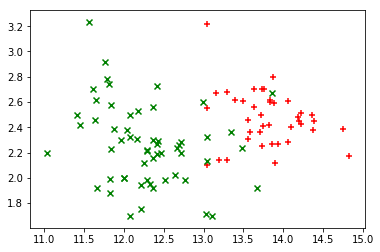
\includegraphics[width=.35\textwidth]{lr2noboundary} \quad \quad  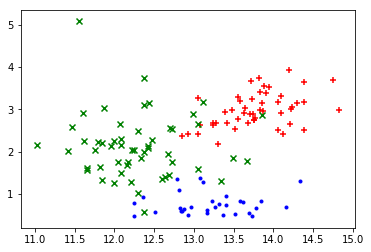
\includegraphics[width=.35\textwidth]{lr3noboundary}
%%	\end{center}
%%\end{figure}
%%Then the decision boundaries given by hyper-planes would be:
%%\begin{figure}[H]
%%	\begin{center}
%%		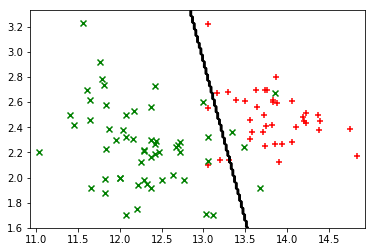
\includegraphics[width=.35\textwidth]{lr2boundary} \quad \quad  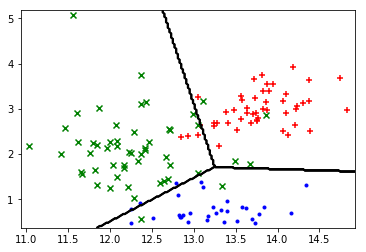
\includegraphics[width=.35\textwidth]{lr3boundary}
%%	\end{center}
%%\end{figure}
%%
%%\break
%%\subsection{How to find these hyper-planes:  logistic regressions}
%%For a collection of subsets $A_1,...,A_k\subset \mathbb{R}^d$, try to find
%%\begin{equation}
%%\label{Wb}
%%W=
%%\begin{pmatrix}
%%w_1\\
%%\vdots\\
%%w_k
%%\end{pmatrix}
%%\in \mathbb{R}^{k\times d},
%%b=
%%\begin{pmatrix}
%%b_1\\
%%\vdots\\
%%b_k
%%\end{pmatrix}
%%\in \mathbb{R}^{k\times d},
%%\end{equation}
%%such that,   for each $1\le i\le k$ and $ j \neq i$
%%\begin{equation}
%%\label{eq:3}
%%(Wx+b)_i > (Wx+b)_j,\ \forall x\in A_i,
%%\end{equation}
%%or
%%\begin{equation}
%%\label{eq:3}
%%w_ix+b_i > w_jx+b_j,\ \forall x\in A_i.
%%\end{equation}
%
%More details of logistic regression will be discussed later.



\break
\section{Some popular data sets in image classification}
In this subsection, we will introduce some popular and standard data sets
in image classification. The most popular four data sets, MNIST, CIFAR-10, CIFAR-100 and ImageNet are shown in Table \ref{popular_dataset}.

\begin{table}[H]
	\centering
	\begin{tabular}{|c|c|c|c|c|c|}
		\hline
		% after \\: \hline or \cline{col1-col2} \cline{col3-col4} ...
		dataset &  training (N) & test (M)   & classes (k) & channels (c)& input size (d)\\\hline
		MNIST	&	60K	&	10K	&	10	& Greyscale & 28*28  \\\hline
		CIFAR-10	&	50K 	&	10K	&	10 & RGB & 32*32   \\\hline
		CIFAR-100	&	50K 	&	10K	&	100 & RGB & 32*32   \\\hline
		ImageNet	&	1.2M 	&	50K	&	1000 &	RGB & 224*224  \\\hline
	\end{tabular}
	\caption{Basic descriptions about popular datasets }
	\label{popular_dataset}
\end{table}

\break
\subsection{MNIST (Modified National Institute of Standards and Technology Database)}
MNIST\cite{lecun1998mnist} is a database for handwritten digits. It is a simple database for people who want to try learning techniques and pattern recognition methods on real-world data while spending minimal efforts on preprocessing and formatting. In order to use MNIST for the classification problem, the following setup is often used:
\begin{itemize}
	\item Training set : $N = 60,000$;
	\item Test set : $M = 10,000$;
	\item Image size : $d =28*28*1=784$;
	\item Classes: $ k = 10$;
\end{itemize}
\begin{figure}[H]
	\begin{center}
		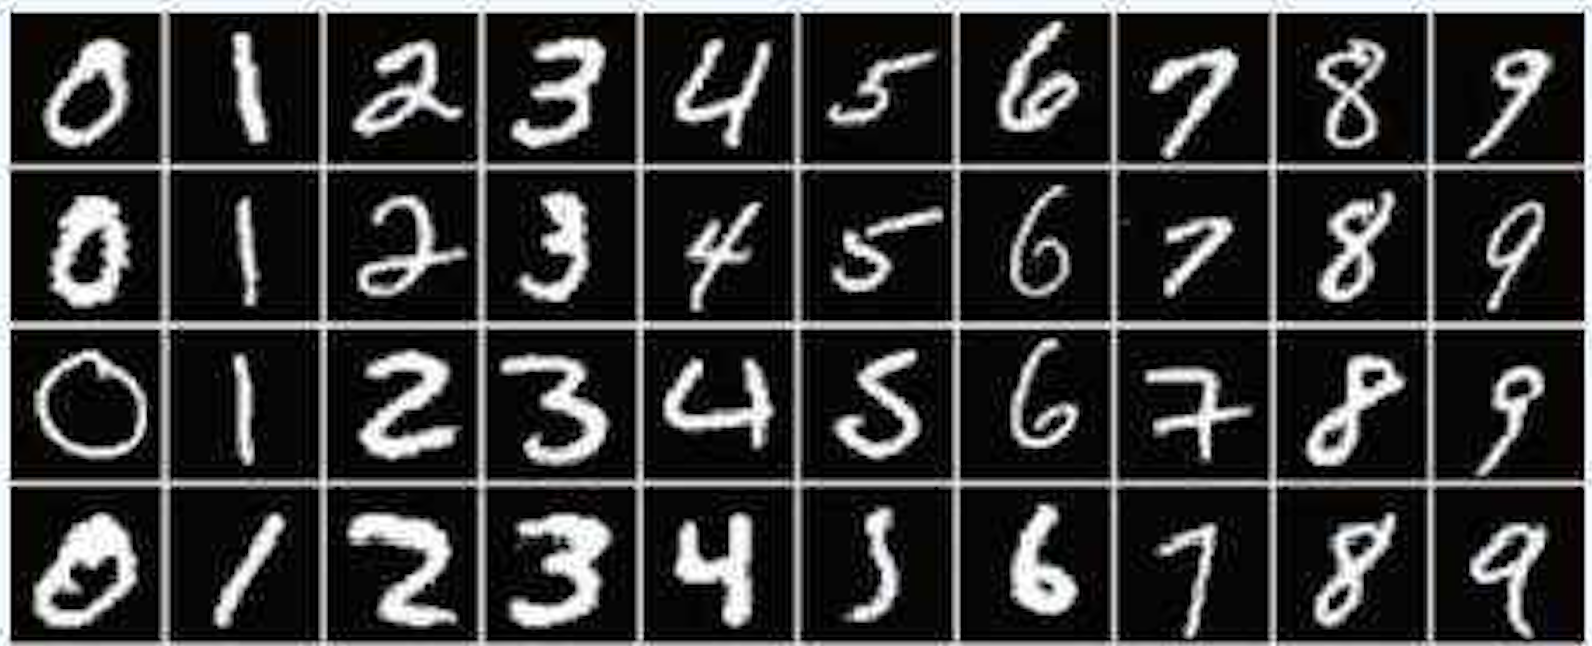
\includegraphics[height=.2\textheight]{mnist_short.png}
		\caption{Some images in MNIST.}
	\end{center}
\end{figure}
The following example shows  an image of handwritten digits is represented mathematically
\break
$$
x=\adjustbox{valign=c}{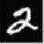
\includegraphics[height=.03\textheight]{mnist2_1.jpg}}
=
\begin{pmatrix}
  x_1\\
x_2\\
\vdots\\
x_{784}
\end{pmatrix}
\in \mathbb R^{784}.
$$
MNIST has 10 classes denoted by $\{A_k\}_{k=1}^{10}$ as shown in the following, where $A_{k}$ is the set of handwritten digits $k$ for $k=1,2,3,...,9$ and $A_{10}$ is the set of handwritten digits $0$
%\begin{equation}
%\label{A1}
%A_1=
%\left\{
%\adjustbox{valign=c}{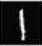
\includegraphics[height=.03\textheight]{mnist1_1.jpg}},
%\adjustbox{valign=c}{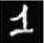
\includegraphics[height=.03\textheight]{mnist1_2.jpg}},
%\adjustbox{valign=c}{
\includegraphics[height=.03\textheight]{mnist1_3.jpg}}, \cdots
%\right\}
%\subset \mathbb R^{784}
%\end{equation}
\begin{equation}
  \label{A2}
A_2=
\left\{
\adjustbox{valign=c}{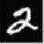
\includegraphics[height=.03\textheight]{mnist2_1.jpg}},
\adjustbox{valign=c}{
\includegraphics[height=.03\textheight]{mnist2_2.jpg}},\cdots
%\adjustbox{valign=c}{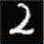
\includegraphics[height=.03\textheight]{mnist2_3.jpg}}, \cdots
\right\},~
%\subset \mathbb R^{784}
A_{9}=
\left\{
\adjustbox{valign=c}{
\includegraphics[height=.03\textheight]{mnist9_1.jpg}},
\adjustbox{valign=c}{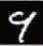
\includegraphics[height=.03\textheight]{mnist9_2.jpg}},\cdots
%\adjustbox{valign=c}{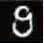
\includegraphics[height=.03\textheight]{mnist9_3.jpg}}, \cdots
\right\},~
A_{10}=
\left\{
\adjustbox{valign=c}{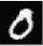
\includegraphics[height=.03\textheight]{mnist0_1.jpg}},
\adjustbox{valign=c}{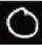
\includegraphics[height=.03\textheight]{mnist0_2.jpg}}, \cdots
%\adjustbox{valign=c}{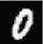
\includegraphics[height=.03\textheight]{mnist0_3.jpg}}, \cdots
\right\}
\subset \mathbb R^{784}.
\end{equation}



\break
\subsection{CIFAR}
\paragraph{CIFAR-10}
CIFAR-10\cite{krizhevsky2009learning} is a set of images that can be used to teach a computer how to recognize objects. It contains 60,000 32x32 color images in 10 different classes,  with 6000 images per class. The 10 different classes represent airplanes, cars, birds, cats, deer, dogs, frogs, horses, ships, and trucks. In order to use CIFAR-10 for the classification problem, people usually use the following setup:
\begin{itemize}
	\item Training set : $N = 50,000$
	\item Test set : $M = 10,000$
	\item Image size : $d  = 32*32*3$
	\item Classes: $k = 10$
\end{itemize}
\begin{figure}[H]
	\begin{center}
		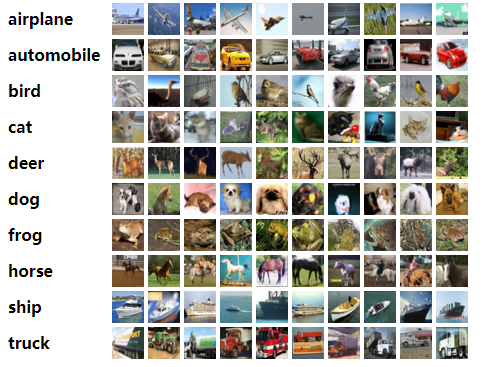
\includegraphics[height=.26\textheight]{cifar10.jpg}
		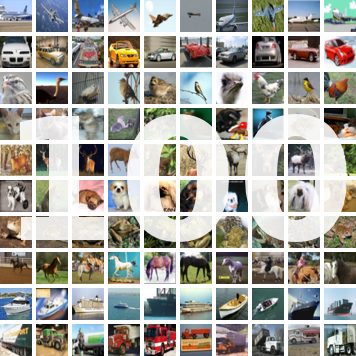
\includegraphics[height=0.26\textheight]{cifar100.png}
		\label{Fig: CIFAR-10}
		\caption{Left: Some images in CIFAR-10. Right: Some images in CIFAR-100.}
	\end{center}
\end{figure}

%\begin{figure}[H]
%	\begin{center}
%		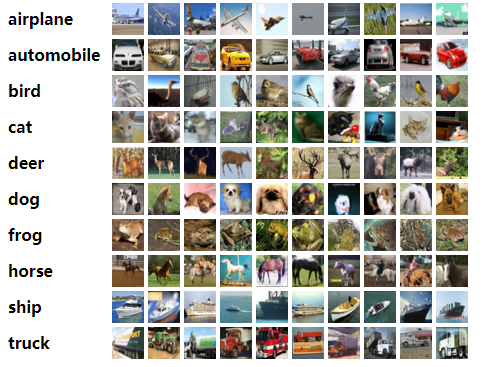
\includegraphics[height=.4\textheight]{cifar10.jpg}
%		\label{Fig: CIFAR-10}
%		\caption{Some images in CIFAR-10.}
%	\end{center}
%\end{figure}
%\begin{figure}[H]
%	\begin{center}
%		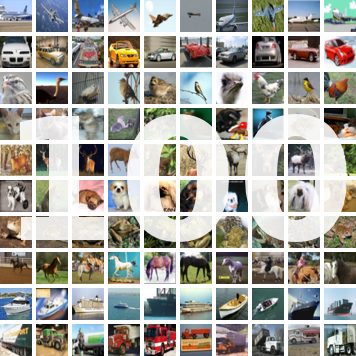
\includegraphics[height=0.35\textheight]{cifar100.png}
%		\caption{Some images in CIFAR-100.}
%	\end{center}
%\end{figure}

\break

\paragraph{CIFAR-100}
CIFAR-100\cite{krizhevsky2009learning} is just like the CIFAR-10, except it has 100 classes containing 600 images each. There are 500 training images and 100 testing images per class. The 100 classes in the CIFAR-100 are grouped into 20 superclasses and each superclass has 5 classes. Each image comes with a ``fine" label (the class to which it belongs) and a ``coarse" label (the superclass to which it belongs). In order to use CIFAR-100 for the classification problem, people usually use the following setup:

\begin{itemize}
	\item Training set : $N = 50,000$
	\item Test set : $M = 10,000$
	\item Image size : $d = 32*32*3$
	\item Classes: $k = 100$
	\end{itemize}
%\begin{figure}[H]
%	\begin{center}
%		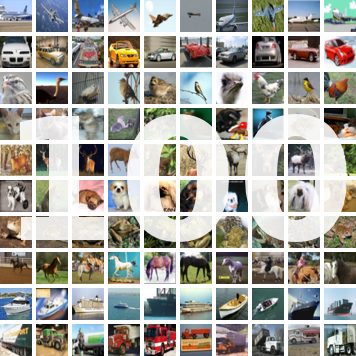
\includegraphics[height=0.35\textheight]{cifar100.png}
%		\caption{Some images in CIFAR-100.}
%	\end{center}
%\end{figure}

\subsection{ImageNet}
The ImageNet\cite{deng2009imagenet} project is a large visual database designed for use in visual object recognition software research. More than 1 million images have been hand labeled to indicate what objects are pictured. It is organized according to the WordNet hierarchy (currently only the nouns), in which each node of the hierarchy is depicted by hundreds and thousands of images.
Since 2010, the ImageNet runs an annual software contest, the ImageNet Large Scale Visual Recognition Challenge (ILSVRC), where software programs compete to correctly classify and detect objects and scenes. In order to use ImageNet for the classification problem, we list the setup of ILSVRC2012 in the following
\begin{itemize}
	\item Training set : $N = 1,200,000$
	\item Test set : $M = 50,000$
	\item Image size : $d = 224*224*3$
	\item Classes: $k = 1,000$
\end{itemize}
%\begin{figure}[H]
%	\begin{center}
%		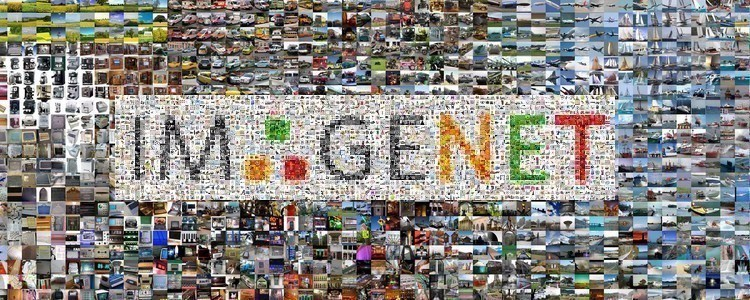
\includegraphics[height=0.25\textheight]{imagenet.jpeg}
%		
%	\end{center}
%\end{figure}


\begin{figure}[H]
	\begin{center}
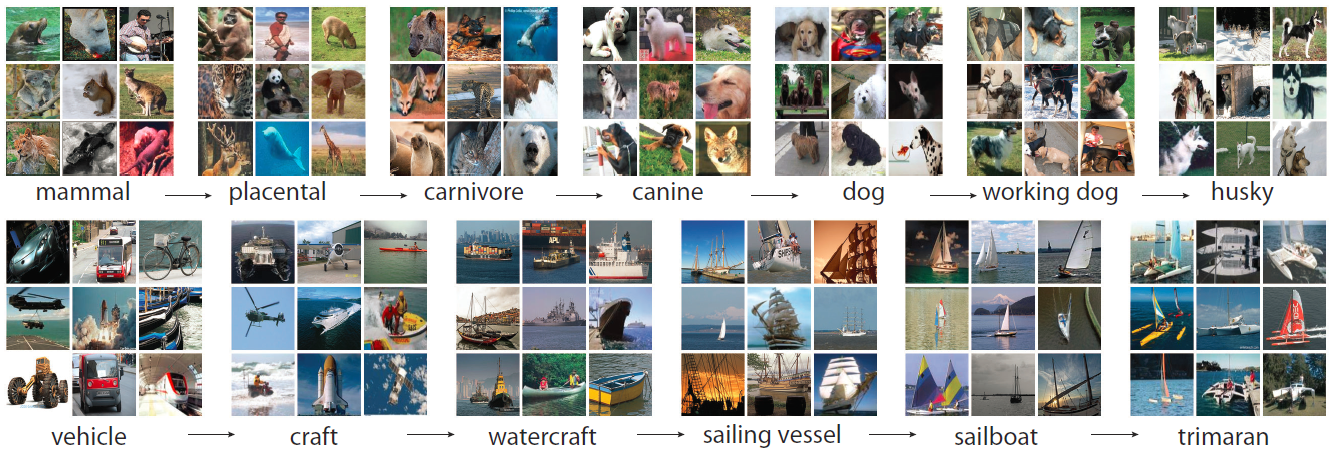
\includegraphics[height=0.22\textheight]{imagenet-example.png}
		\caption{Some images in ImageNet.}
	\end{center}
\end{figure}


\break
%\section{Classification and decision boundaries}
%A classification problem is to find some curves or surfaces to separate some sets of data. As examples, the following two images show how a circle and a curve separate different sets of points
%\begin{figure}[H]
%	\begin{center}
%		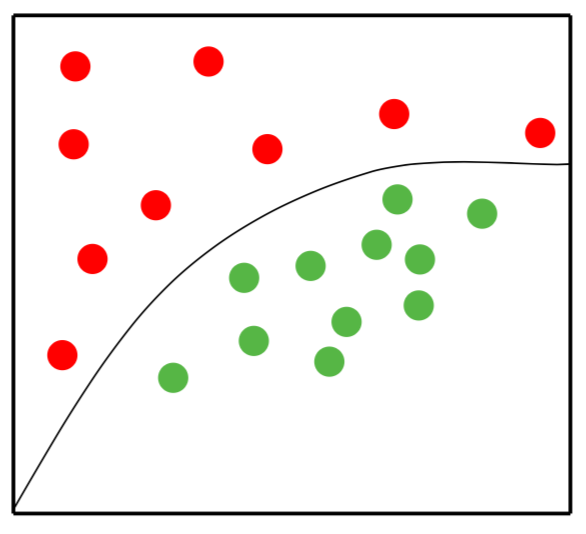
\includegraphics[width=1.5in]{NLinearS1.png}  \quad
%                \quad  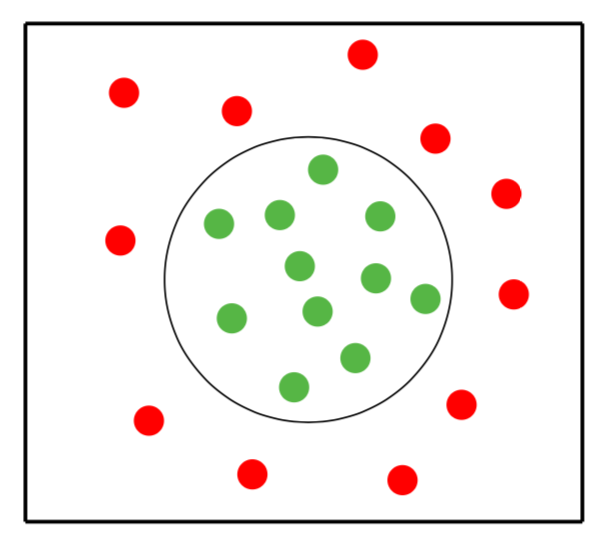
\includegraphics[width=1.5in]{NLinearS2.png}
%	\end{center}
%\end{figure}

%\begin{figure}[H]
%	\begin{center}
%		 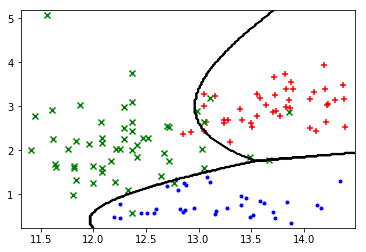
\includegraphics[width=.35\textwidth,
%                 height=0.3\textheight]{nlr3boundary}
%	\end{center}
%\end{figure}
%\input{Jianqing}
